\chapter{The $\lambda$-calculus and Curry Type Assignment System Implementation in Java}
The Java version of implementation is transferred directly from Haskell. However, the semantics and operational order of Haskell is difference from Java, especially the `where' statement of Haskell. The 'where' declaration is called when the defined variables are used, however, in Java, we need to separate a `where' block into parts according to where it is called. An example is shown in Section \ref{sec:hj}. This differece is worth taking care of when transfer the Haskell into Java, otherwise, NullPointerException may occur. 

In all data types, the method toString() has been implemented -- more precisely overridden, as it is a method of the Java primary class\verb| Object|. This function is used to print out the data type as a string. There are more method signatures defined in the interfaces as a reference to instantiable classes. 

\section{Different operational order between Haskell and Java}{\label{sec:hj}}
As mentioned above, the operaional order of Haskell is different from Java, not only the pattern matching, but also the `where' declarations. Since the code in Haskell cannot be transferred into Java directly, it largely abandoned the simplicity of codes. Following is a piece of code that defines principle pair algorithm:
\begin{verbatim}
ppc :: Term -> [Char] -> (PPc, [Char])
ppc (Abs x y) r | contains (Var x) pi = ((removeItem (Var x, a) pi, (TP a p)), tl1)
                | otherwise = ((pi, (TP f p)), tl1)
                            where (f, tl) = fresh r                    (1) 
                                  ((pi, p), tl1) = ppc y tl            (2)
                                  (_, a) = search (Var x) pi           (3)

\end{verbatim}

`Guards' are used as an if-then-else block. There are three declarations in the `where' block each with a distinct number. For the first condition of ppc function, declaration (1)(2)(3) are called since all the declared variables are used. In the `otherwise' condition, only declaration (1)(2) are called. In this case, in order to transfer the Haskell function into Java methods, we need to repetitively define the variables which largely reduces the simplicity of codes. 





\begin{verbatim}
public PPC ppc(Term term, String counter){
     ...
     else if(term instanceof Abstraction){
        Variable xv = new Variable(((Abstraction) term).getName());
        PPC receiver = ppc(((Abstraction) term).getTerm(), counter);
        if(receiver != null){
           if(contains(xv, receiver.getSubject())){
             Type searchType = search(xv, receiver.getSubject()).getPredicate();
             ArrayList<Statement> original = receiver.getSubject().getContext();
             ArrayList<Statement> remove = new ArrayList<>();

             for(Statement s: original){
               if(s.getSubject().equals(xv)) remove.add(s);
             }

             for(Statement rm: remove){
                original.remove(rm);
             }

             TP tp = new TP(searchType, receiver.getPredicate());
             return new PPC(new Context(original), tp, receiver.getCounter());
          }
          else{
             TVar f = new TVar(receiver.getCounter().substring(0, 1));
             return new PPC(receiver.getSubject(), new TP(f, receiver.getPredicate()),
                            receiver.getCounter().substring(1));

          }
       }
       else {
           return null;
       }
     }
     ...
}
\end{verbatim}

\section{$\lambda$-calculus Representation}
\subsection{$\lambda$-terms}
A Lambda term can either be a variable, an abstraction or an application. An interface `Term' is defined as a reference type, which has three lambda term implementations. This is the generic representation of all lambda terms.

\begin{figure}[ht]
\centering
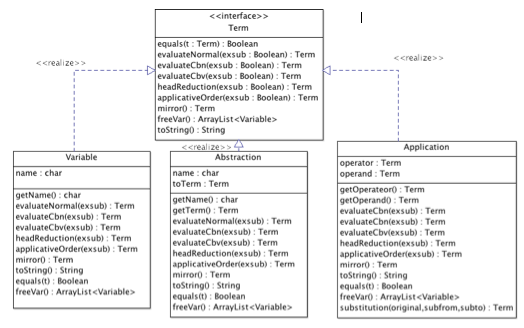
\includegraphics[scale=0.7]{pics/Term}
\caption{Class diagram of Lambda Calculus data structures}
\label{fig:term1}
\end{figure}

This interface defines the method \verb|equals(Term t)|, which return a boolean states whether it is equal to the input term. This method overrides the \verb|equals(Object o)| method of the Java primary class \verb|Object|. It is essential in the reduction procedure, since we can decide whether a term is reducible by compare the term before reduction and after. If the term is the same as it before reduction, then it cannot be reduced. Therefore, we know when we can stop the reduction procedure.  

As mentioned in Section \ref{sec:reductionstrategy}, there are five reduction strategies enabled in the reducer. So there are five method signatures defined in the interface: \textsf{evaluateNormal(Bool exsub), evaluateCbn(Bool exsub), evaluateCbv(Bool exsub), headReduction(Bool exsub), applicativeOrder(Bool exsub)}. Each of these method refers to a specific reduction strategy as the method name. 

The method \textsf{mirror()} is used to create a mirror term with exactly the same class variables. This method is used when the substitution is performed. For example, if we have a lambda term $\lambda f.(\lambda x.f(xx))(\lambda x.f(xx))$, it is reduced to $\lambda f.f((\lambda x.f(xx))(\lambda x.f(xx)))$. If we do not create a mirror term of $(\lambda x.f(xx))$, both of these two $(\lambda x.f(xx))$ would refer to the same memory space. In other words, the abstraction $(\lambda x.f(xx))$ is used twice to form an application. Therefore, if operations performed on the function, it is also performed on the argument. It is essential to create a mirror term that separate those two terms although they look exactly the same.      

Finally, the \textsf{toString()} method of class \textsf{Object} is overridden to transform a lambda term to a string. 

Notice that, in the implementation class \verb|Application|, there is a \textsf{substitution(Term original, Term subfrom, Term subto):Term} method. It is used to substitute bound variables in an abstraction, which is an application function, to the argument. The first parameter of the method is the body of abstraction, the second argument states which bound variable could be substituted and the third argument states what it could be substituted to.

\subsection{Interpreter}
To allow interactions and inputs from users, the program needs to interpret the input term into a data structure in the system. Figure \ref{fig:inter} illustrates all the methods that used to interpret an input into a lambda term data structure.   

\begin{figure}[ht]
\centering
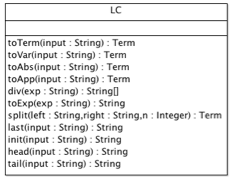
\includegraphics[scale=0.6]{pics/LC}
\caption{Interpretation methods in LC class}
\label{fig:inter}
\end{figure}

The method \textsf{toTerm(String input)} takes a string as input and returns a \textsf{Term}. It calls \textsf{toVar(String input), toAbs(String input)} or \textsf{toApp(String input)} according to type of the outermost term. Then, those three methods iteratively call each other until the whole term is interpreted.   

\textsf{div(String exp)} divides an application into the function and argument. Basically, it return an array with 2 string elements. The method \textsf{toExp(String exp)} is used to remove brackets of applications and returns an expression that is bracker-free. Finally, the most important method \textsf{split(String left, String right, Int n)} implements the bracket removal mechanism. It marks the right most right bracker `)' and find the matching left bracket `(' and extract the term out without brackets.

Since the Java implementation is directly transferred from Haskell, there are also four basic string operations which are Haskell builit-in functions. \textsf{last(String input)} takes a string and returns the last character of the string, it returns itself if the length of input string is 1. \textsf{init(String input)} accepts a string and returns the string without its last character, it returns an empty string if it only contains one character. \textsf{head(String input)} takes a string and returns the first element of the string, it returns itself when the input string length is 1. \textsf{tail(String input)} takes a string and returns the string without its first element, it returns an empty string when the length of input is 1. 

Following is the example of how those Haskell built-in function work:

\begin{verbatim}
              init "Hello"   "Hell"            head "Haskell"   "H" 
              init "A"       ""                head "A"         "A"
\end{verbatim}

\begin{verbatim}
              last "String"   "g"              tail "Lambda"   "ambda" 
              last "A"        "A"              tail "A"         ""
\end{verbatim}


\section{Curry Type Assignment System Representation}





\subsection{Type variable and Type}

\begin{figure}[ht]
\centering
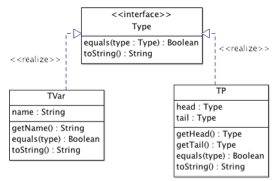
\includegraphics[scale=0.7]{pics/Type}
\caption{type}
\label{fig:type}
\end{figure}

A type variable is a single type that ranged from A to Z. A type is represented as a tree structure. For example, the type $(A\rightarrow B)\rightarrow C$ is represented as \textsf{TP(TP (TVar A)(TVar B))(TVar C)}. Or in a more intuitionistic way:

\Tree [.TP [.TP A B ] C ]



\subsection{Type substitution}

\begin{figure}[ht]
\centering
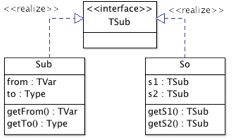
\includegraphics[scale=0.7]{pics/TSub}
\caption{Class diagram of Lambda Calculus data structures}
\label{fig:term1}
\end{figure}


\begin{figure}[ht]
\centering
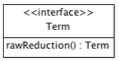
\includegraphics[scale=0.7]{pics/TermRaw}
\caption{Class diagram of Lambda Calculus data structures}
\label{fig:term1}
\end{figure}


\begin{figure}
\centering
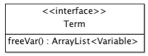
\includegraphics[scale=0.7]{pics/TermType}
\caption{Class diagram of Lambda Calculus data structures}
\label{fig:term1}
\end{figure}



\begin{figure}
\centering
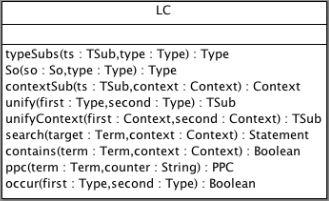
\includegraphics[scale=0.6]{pics/LCType}
\caption{Class diagram of Lambda Calculus data structures}
\label{fig:term1}
\end{figure}


\begin{figure}
\centering
\begin{minipage}{.3\textwidth}
\centering
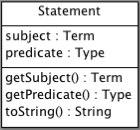
\includegraphics[scale=0.8]{pics/Statement}
\caption{Caption for figure 1}
\label{fig:test1}
\end{minipage}\hfill
\begin{minipage}{.3\textwidth}
\centering
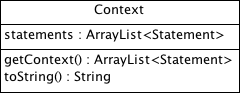
\includegraphics[scale=0.65]{pics/Context}
\caption{Caption for figure 2}
\label{fig:test2}
\end{minipage}\hfill
\begin{minipage}{.3\textwidth}
\centering
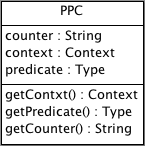
\includegraphics[scale=0.7]{pics/PPC}
\caption{Caption for figure 3}
\label{fig:test3}
\end{minipage}
\end{figure}


\section{Auxiliary Functions}

\section{Syntax and Interpreter}